\documentclass{report}
\usepackage[utf8x]{inputenc}
\usepackage[T1]{fontenc}
\usepackage[francais]{babel}
\usepackage{graphicx}
\usepackage{hyperref}
\author{Léo Unbekandt - Guillaume Paran - Lucas Saurel}
\date{Mai 2012}
\title{Projet web - UnsapaIPW}

\begin{document}

  \maketitle
  \tableofcontents

  \section*{Introduction}
  \addcontentsline{toc}{section}{Introduction}

  \section{Fonctionnalités de l'application}
  \section{Organisation de l'équipe}
  \section{Schéma de données}
    Le sujet nous imposait d'utiliser un certain nombre
    auxquels nous avons ajouté un certain nombre d'attributs.

    \begin{figure}
      \caption{Schéma relationnel}
      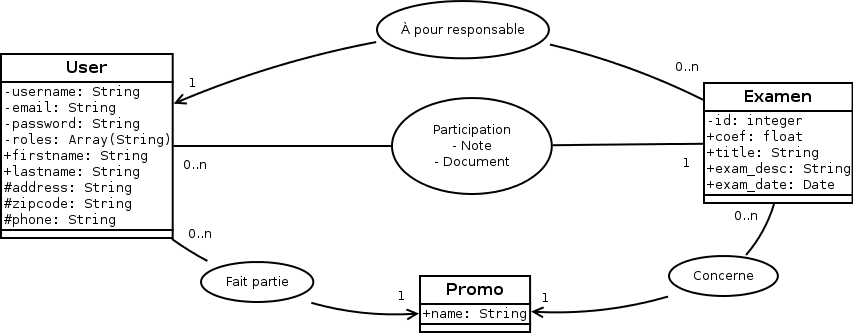
\includegraphics[width=0.9\textwidth]{./data.png}
    \end{figure}

    \begin{figure}
      \caption{Modèle physique de base de données}
      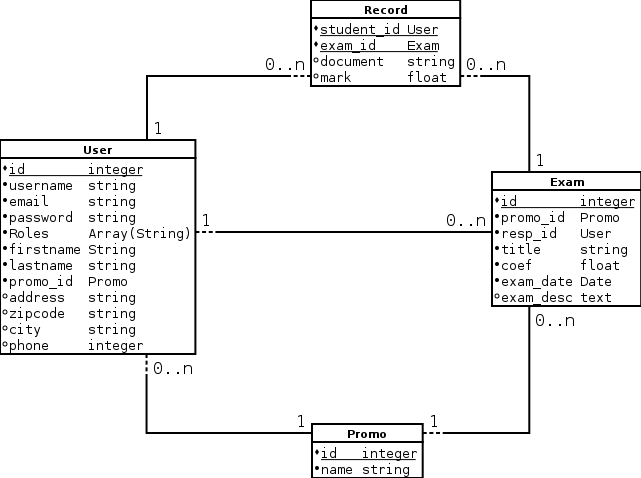
\includegraphics[width=0.9\textwidth]{./db.png}
    \end{figure}

    \subsection{User}
      En plus des champs prérequis :
      \begin{itemize}
        \item{Prénom}
        \item{Nom}
        \item{Adresse}
        \item{Code postal}
        \item{Ville}
        \item{Adresse e-mail}
        \item{Numéro de téléphone}
      \end{itemize}

      Le UserBundle nous rajoute toute la partie nécessaire à la gestion de
      l'utilisateur côté serveur.
      \begin{itemize}
        \item{Le mot de passe $\Rightarrow$ chiffré en sha1 dans la BDD}
        \item{Les rôles $\Rightarrow$ Pour la gestion des permissions}
        \item{Nom d'utilisateur}
        \item{Expiration du compte, confirmation par email etc.}
      \end{itemize}

      Et enfin nous avons ajouté un champs pour notre besoin qui est une
      promotion, en effet, on considère qu'un étudiant appartient à une
      promotion précise.

    \subsection{Promo}
      Les promotions correspondent à un regroupement d'utilisateur, dans le
      cas d'utilisation présent, tous les étudiants d'une même année 
      appartiennent à une promotion unique.

    \subsection{Exam}
      Un examen représente une épreuve définie par un enseignant. L'examen 
			comprend les propriétés suivantes :
			\begin{itemize}
				\item{Titre}
				\item{Descrption}
				\item{Promotion}
				\item{Coefficient}
				\item{Date limite}
				\item{Responsable : Un user responsable de TD}
			\end{itemize}
			Par défaut, lors de la création de l'examen, tous les étudiants de la
			promotion sélectionnée sont concernés par l'examen, mais il est également possible
			de modifier au cas par cas si un étudiant est affecté par l'examen.
    \subsection{Record}
			L'entité Record fait le lien entre les étudiants et les examens. En effet dans un record
			on attribue pour un étudiant et un examen, la note, ainsi que le document rendu 
			(Fichier pdf ou word).

			On a donc :
			\begin{itemize}
				\item{Étudiant}
				\item{Examen}
				\item{Note}
				\item{Document}
			\end{itemize}

			Ainsi un Record avec la note et le document NULL, correspond au fait qu'un étudiant doit
			effectuer un rendu pour un tel examen. Quand il rend quelque chose, on peuple le champs
			'Document'. Et ensuite quand l'examen est terminé le responsable de l'examen peut associer 
			une note.


  \section{Réalisation Technique}
    \subsection{UserBundle}
      Nous avons utilisé un Bundle d'extension nommé : 
      \href{https://github.com/FriendsOfSymfony/FOSUserBundle}{UserBundle}.
      
      Ce bundle constitue la brique applicative qui permet d'effectuer toutes
      les actions nécessaires à presque tous les projets, c'est-à-dire :
      \begin{itemize}
        \item{Inscription}
        \item{Authentification}
        \item{Connexion}
        \item{Déconnexion}
        \item{Gestion du profil}
        \item{Changement de mot de passe}
      \end{itemize}
      Nous évitant du travail laborieux qui ne sert pas sur le plan métier de
      l'application.

    \subsection{Les tests avec PHPUnit}
			Nous avons principalement testé les différentes entités. Grâce à PHPUnit nous
			avons généré la couverture en tests de notre code.

			\href{http://ares-ensiie.eu/~unbekandt2011/UnsapaIPW/cov}{Couverture des tests}
    \subsection{La documentation développeur avec phpDocumentor}
			Tout notre code a été documenté en utilisant phpDocumentor. On peut trouvé cette
			documentation à l'adresse :

			\href{http://ares-ensiie.eu/~unbekandt2011/UnsapaIPW/doc}{Documentation développeur}

  \section*{Conclusion}
  \addcontentsline{toc}{section}{Conclusion}

\end{document}
